\documentclass[11pt,handout,pdf,hyperref={unicode}]{beamer}

\usepackage{fontspec}

\usepackage{pgfpages}
%\usepackage[utf8]{inputenc}
%\usepackage[english,russian]{babel}
%\usepackage{graphicx}
%\usepackage{pagenumber}
\usepackage{xltxtra}
\usepackage{xunicode}

% Fonts
\setsansfont{Liberation Sans}
\setmainfont{Times New Roman}
\newfontfamily{\cyrillicfont}{Times New Roman}
\setmonofont{DejaVu Sans Mono}
\newfontfamily{\cyrillicfonttt}{DejaVu Sans Mono}
\usepackage{polyglossia}
\setmainlanguage{russian} 
\setotherlanguage{english}

\usepackage{minted}

\defbeamertemplate*{footline}{Warsaw} {%
\leavevmode%
\hbox{%
\begin{beamercolorbox}[wd=.5\paperwidth,ht=2.5ex,dp=1.125ex,leftskip=.3cm,rightskip=.3cm]{author in head/foot}%
\insertframenumber{}%
\hfill\insertshortauthor
\end{beamercolorbox}%
\begin{beamercolorbox}[wd=.5\paperwidth,ht=2.5ex,dp=1.125ex,leftskip=.3cm,rightskip=.3cm]{title in head/foot}%
\usebeamerfont{title in head/foot}\insertshorttitle
\end{beamercolorbox}
}%
\vskip0pt%
}

\begin{document}
\pagestyle{plain}

\begin{frame}

\texttt{ }

\texttt{ Язык Ride - простой функциональный язык смарт-смартактов. }

\texttt{ }

\texttt{ Михаил Потанин. }

\texttt{ Scala-разработчик Waves Platform. }

\texttt{ mpotanin@wavesplatform.com }

\end{frame}

\begin{frame}

\texttt{ Язык Ride это язык смарт-контрактов в блокчейне Waves. }

\end{frame}

\begin{frame}

\texttt{ }

\texttt{ Язык Ride это язык смарт-контрактов в блокчейне Waves. }

\texttt{ }

\texttt{ Язык очень простой }

\end{frame}


\begin{frame}[fragile]

\texttt{ Простой синтаксис. }

\texttt{ }

\begin{minted}[fontsize=\small]{ride}

let alicePubKey  =
        base58'5Azf.....VdEpMM'
let bobPubKey    =
        base58'2KwU.....wi2VDF'
let cooperPubKey =
        base58'GbrU.....mgt5cD'

func check(proof: Int, key: ByteVector) =
  if sigVerify(tx.bodyBytes, tx.proofs[proof], key)
  then 1
  else 0

#check whoever provided the valid proof
let aliceSigned  = check(0, alicePubKey)
let bobSigned    = check(1, bobPubKey)
let cooperSigned = check(2, cooperPubKey)

#sum up every valid proof to get at least 2
aliceSigned + bobSigned + cooperSigned >= 2

\end{minted}
\end{frame}

\begin{frame}[fragile]

\texttt{ Что такое смарт-контракты? }

\end{frame}

\begin{frame}[fragile]

\texttt{ Что такое смарт-контракты? }

\texttt{ }

\texttt{ Договор, оформленный в виде кода. }

\texttt{ Концепцию предложил Ник Сабо в 1996 году для удешевления составления договоров для микроплатежей. }

\end{frame}

\begin{frame}[fragile]

\texttt{ Основное применение смарт-контрактов в настоящее время - блокчейн. }

\end{frame}

\begin{frame}[fragile]

\texttt{ Основное применение смарт-контрактов в настоящее время - блокчейн. }

\texttt{ }

\texttt{ Но ничто не мешает применять их более широко: }

\texttt{ }

\texttt{ В банковской сфере можно формально описать условия выплат. }

\end{frame}

\begin{frame}[fragile]

\texttt{ Основное применение смарт-контрактов в настоящее время - блокчейн. }

\texttt{ }

\texttt{ Но ничто не мешает применять их более широко: }

\texttt{ }

\texttt{ В банковской сфере можно формально описать условия выплат. }

\texttt{ }

\texttt{ В многопользовательских играх с развитой экономикой. }

\end{frame}

\begin{frame}[fragile]

\texttt{ К какой информации имеет доступ смарт-контракт и какие действия он может инициировать? }

\end{frame}

\begin{frame}[fragile]

\texttt{ К какой информации имеет доступ смарт-контракт и какие действия он может инициировать? }

\texttt{ }

\texttt{ В игре он может иметь доступ ко всем элементам игровой вселенной, которые разрешены правилами игры. }

\end{frame}

\begin{frame}[fragile]

\texttt{ К какой информации имеет доступ смарт-контракт и какие действия он может инициировать? }

\texttt{ }

\texttt{ В игре он может иметь доступ ко всем элементам игровой вселенной, которые разрешены правилами игры. }

\texttt{ }

\texttt{ Для банков - это данные из различных реестров и введенные оператором. }

\end{frame}

\begin{frame}[fragile]

\texttt{ К какой информации имеет доступ смарт-контракт и какие действия он может инициировать? }

\texttt{ }

\texttt{ В игре он может иметь доступ ко всем элементам игровой вселенной, которые разрешены правилами игры. }

\texttt{ }

\texttt{ Для банков - это данные из различных реестров и введенные оператором. }

\texttt{ }

\texttt{ В блокчейне это только данные самого блокчейна или помещенные в блокчейн довереннымой третьей стороной (оракулом). }

\end{frame}

\begin{frame}[fragile]

\texttt{ Кто пишет смарт-контракты. }

\end{frame}

\begin{frame}[fragile]

\texttt{ Кто пишет смарт-контракты. }

\texttt{ }

\texttt{ Сейчас это обычные программисты. }

\end{frame}

\begin{frame}[fragile]

\texttt{ Кто пишет смарт-контракты. }

\texttt{ }

\texttt{ Сейчас это обычные программисты. }

\texttt{ }

\texttt{ В идеале, это юристы и владельцы бизнесов. }

\end{frame}

\begin{frame}[fragile]

\texttt{ Цена ошибки. }

\end{frame}

\begin{frame}[fragile]

\texttt{ Цена ошибки. }

\texttt{ }

\texttt{ В результате программисткой ошибки в смарт-контракте пользователь может потерять деньги. }

\end{frame}

\begin{frame}[fragile]

\texttt{ Цена ошибки. }

\texttt{ }

\texttt{ В результате программисткой ошибки в смарт-контракте пользователь может потерять деньги. }

\texttt{ }

\texttt{ К счету пользователя может получить доступ злоумышленник. }

\end{frame}

\begin{frame}[fragile]

\texttt{ Цена ошибки. }

\texttt{ }

\texttt{ В результате программисткой ошибки в смарт-контракте пользователь может потерять деньги. }

\texttt{ }

\texttt{ К счету пользователя может получить доступ злоумышленник. }

\texttt{ }

\texttt{ Счет может оказаться заблокирован. }

\end{frame}

\begin{frame}[fragile]

\texttt{ Как уменьшить вероятность ошибок? }

\end{frame}

\begin{frame}[fragile]

\texttt{ Как уменьшить вероятность ошибок? }

\texttt{ }

\texttt{ Классический ответ - тестирование. }

\end{frame}

\begin{frame}[fragile]

\texttt{ Как уменьшить вероятность ошибок? }

\texttt{ }

\texttt{ Классический ответ - тестирование. }

\texttt{ }

\texttt{ Тестировать смарт-контракты необходимо, но это не панацея. }

\end{frame}

\begin{frame}[fragile]

\texttt{ Как уменьшить вероятность ошибок? }

\texttt{ }

\texttt{ Что может предложить язык. }

\end{frame}

\begin{frame}[fragile]

\texttt{ Как уменьшить вероятность ошибок? }

\texttt{ }

\texttt{ Что может предложить язык. }

\texttt{ }

\texttt{ Иммутабельность и отсутствие побочных эффектов. }

\end{frame}

\begin{frame}[fragile]

\texttt{ Как уменьшить вероятность ошибок? }

\texttt{ }

\texttt{ Что может предложить язык. }

\texttt{ }

\texttt{ Иммутабельность и отсутствие побочных эффектов. }

\texttt{ }

\texttt{ Статическая типизация. }

\end{frame}

\begin{frame}[fragile]

\texttt{ Как уменьшить вероятность ошибок? }

\texttt{ }

\texttt{ Что может предложить язык. }

\texttt{ }

\texttt{ Иммутабельность и отсутствие побочных эффектов. }

\texttt{ }

\texttt{ Статическая типизация: в Ride реализованы union-типы. }

\end{frame}

\begin{frame}[fragile]

\texttt{ Union-типы. }

\texttt{ }

\begin{minted}[fontsize=\small]{ride}

func incOrSize(v: Int | String) = match v {
   case a: Int    => a+1
   case b: String => size(b)
}

\end{minted}

\end{frame}

\begin{frame}[fragile]

\texttt{ Union-типы. }

\texttt{ }

\begin{minted}[fontsize=\small]{ride}

match getInteger(tx.sender, "p14") {
   case _: Unit => 0
   case v: Int  => v
}

\end{minted}

\end{frame}

\begin{frame}[fragile]

\texttt{ Как уменьшить вероятность ошибок? }

\texttt{ }

\texttt{ Что может предложить язык. }

\texttt{ }

\texttt{ Иммутабельность и отсутствие побочных эффектов. }

\texttt{ }

\texttt{ Статическая типизация: в Ride реализованы union-типы. }

\texttt{ }

\texttt{ Формальная верификация. }

\end{frame}

\begin{frame}[fragile]

\texttt{ Как уменьшить вероятность ошибок? }

\texttt{ }

\texttt{ Формальная верификация. }

\texttt{ }

\texttt{ Благодоря простоте появились внешние проекты }

\end{frame}

\begin{frame}[fragile]

\texttt{ Формальная верификация. }

\texttt{ }

\texttt{ https://habr.com/en/post/450016/ }
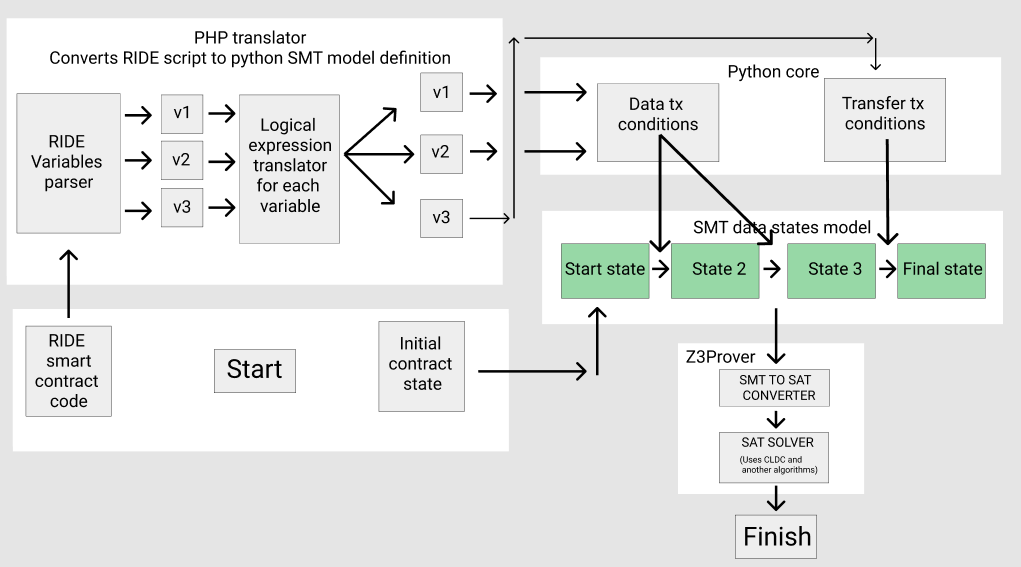
\includegraphics[scale=0.25]{ride_z3.png}

\end{frame}

\begin{frame}[fragile]

\texttt{ Модель выполнения Ride. }

\end{frame}

\begin{frame}[fragile]

\texttt{ Модель выполнения Ride. }

\texttt{ }

\texttt{ Валидация транзакций. }

\end{frame}

\begin{frame}[fragile]

\texttt{ Модель выполнения Ride. }

\texttt{ }

\texttt{ Валидация транзакций. }

\texttt{ }

\texttt{ Контракт это функция из транзакции и текущего состояния блокчейна в булевский тип }

\texttt{ }

\begin{minted}[fontsize=\small]{ocaml}
 contract : Transaction -> Blockchain -> Boolean
\end{minted}

\end{frame}

\begin{frame}[fragile]

\texttt{ Ошибки времени исполнения. }

\end{frame}

\begin{frame}[fragile]

\texttt{ Ошибки времени исполнения. }

\texttt{ }

\texttt{ Ошибки приводят к завершению контракта. Тразнакция в этом случае отклоняется. }

\end{frame}

\begin{frame}[fragile]

\texttt{ Ошибки времени исполнения. }

\texttt{ }

\texttt{ Ошибки приводят к завершению контракта. Тразнакция в этом случае отклоняется. }

\texttt{ }

\texttt{ Возможности обработки ошибок не предусмотрено. }

\end{frame}

\begin{frame}[fragile]

\texttt{ Ошибки в подвыражениях и ленивость. }

\texttt{ }

\begin{minted}{ride}
let x = 1/0
true
\end{minted}

\end{frame}

\begin{frame}[fragile]

\texttt{ Ошибки в подвыражениях и ленивость. }

\texttt{ }

\begin{minted}{ride}
let x = 1/0
true
\end{minted}

\texttt{ }

\texttt{ вычисляется в true, потому что к x нет обращений. }

\end{frame}

\begin{frame}[fragile]

\texttt{ Неполнота по Тьюрингу. }

\end{frame}

\begin{frame}[fragile]

\texttt{ Неполнота по Тьюрингу. }

\texttt{ }

\texttt{ В Ride запрещена рекурсия. }

\end{frame}

\begin{frame}[fragile]

\texttt{ Неполнота по Тьюрингу. }

\texttt{ }

\texttt{ В Ride запрещена рекурсия. }

\texttt{ }

\texttt{ В Ride нет функций высших порядков. }

\end{frame}

\begin{frame}[fragile]

\texttt{ Последовательность операций. }

\end{frame}

\begin{frame}[fragile]

\texttt{ Последовательность операций. }

\texttt{ }

\texttt{ Поведение смарт-контракта может зависеть от сохраненных ранее данных. }

\end{frame}

\begin{frame}[fragile]

\texttt{ Последовательность операций. }

\texttt{ }

\texttt{ Поведение смарт-контракта может зависеть от сохраненных ранее данных. }

\texttt{ }

\texttt{ Сохранение данных - специальный вид транзакции, который тоже проверяется смарт-контрактом. }

\end{frame}

\begin{frame}[fragile]

\texttt{ Последовательность операций. }

\texttt{ }

\texttt{ Поведение смарт-контракта может зависеть от сохраненных ранее данных. }

\texttt{ }

\texttt{ Сохранение данных - специальный вид транзакции, который тоже проверяется смарт-контрактом. }

\texttt{ }

\texttt{ Смарт-контракт может валидировать каждый шаг бизнес-процесса. }

\end{frame}

\begin{frame}[fragile]

\texttt{ Бизнес-процесс часто можно описать в простой формальной модели - конечного автомата или сети Петри. }

\end{frame}

\begin{frame}[fragile]

\texttt{ Бизнес-процесс часто можно описать в простой формальной модели - конечного автомата или сети Петри. }

\texttt{ }

\texttt{ Которые легко реализуются смарт-контрактом. }

\end{frame}

\begin{frame}[fragile]
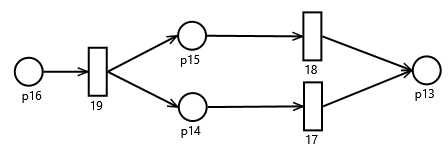
\includegraphics[scale=0.8]{petri_sample.png}

\end{frame}

\begin{frame}[fragile]

\begin{minted}[fontsize=\tiny]{ride}
match tx {
   case tx: DataTransaction => 
     let action = getInteger(tx.data, "action")
         if action == 17 && size(tx.data) == 3
       then
         let p14 = match getInteger(tx.sender, "p14") { case _:Unit => 0 case v: Int => v }
         let p13 = match getInteger(tx.sender, "p13") { case _:Unit => 0 case v: Int => v }
            p14 >= 1 && p14 + -1 == extract(getInteger(tx.data, "p14"))
                     && p13 + 1 == extract(getInteger(tx.data, "p13"))
       else if action == 18 && size(tx.data) == 3
       then
         let p15 = match getInteger(tx.sender, "p15") { case _:Unit => 0 case v: Int => v }
         let p13 = match getInteger(tx.sender, "p13") { case _:Unit => 0 case v: Int => v }
            p15 >= 1 && p15 + -1 == extract(getInteger(tx.data, "p15"))
                     && p13 + 1 == extract(getInteger(tx.data, "p13"))
       else if action == 19 && size(tx.data) == 4
       then
         let p14 = match getInteger(tx.sender, "p14") { case _:Unit => 0 case v: Int => v }
         let p15 = match getInteger(tx.sender, "p15") { case _:Unit => 0 case v: Int => v }
         let p16 = match getInteger(tx.sender, "p16") { case _:Unit => 0 case v: Int => v }
            p16 >= 1 && p14 + 1 == extract(getInteger(tx.data, "p14"))
                     && p15 + 1 == extract(getInteger(tx.data, "p15"))
                     && p16 + -1 == extract(getInteger(tx.data, "p16"))
       else throw("Action is not implemented")
    case tx =>
         true
}
\end{minted}

\end{frame}

\begin{frame}[fragile]

\texttt{ Один вызов смарт-контракта может соответствовать шагу более сложной формальной системы. }

\end{frame}

\begin{frame}[fragile]

\texttt{ Один вызов смарт-контракта может соответствовать шагу более сложной формальной системы. }

\texttt{ В том числе тьюринг-полной. }

\end{frame}

\begin{frame}[fragile]

\texttt{ Один вызов смарт-контракта может соответствовать шагу более сложной формальной системы. }

\texttt{ }

\texttt{ В том числе тьюринг-полной. }

\texttt{ }

\texttt{ Подробно описано на примере Ergo в статье  Александра Чепурного, Василия Харина и Дмитрия Мешкова. }

\texttt{ }

\texttt{ "Self-Reproducing Coins as Universal Turing Machine" }

\texttt{ https://arxiv.org/pdf/1806.10116.pdf }

\end{frame}

\begin{frame}[fragile]

\texttt{ Разделяя приложение на производящий вычисления клиент и валидирующий смарт-контракт можно реализовать любой DApp. }

\end{frame}

\begin{frame}[fragile]

\texttt{ Разделяя приложение на производящий вычисления клиент и валидирующий смарт-контракт можно реализовать любой DApp. }

\texttt{ }

\texttt{ Но сложно. }

\end{frame}

\begin{frame}[fragile]

\texttt{ Разделяя приложение на производящий вычисления клиент и валидирующий смарт-контракт можно реализовать любой DApp. }

\texttt{ }

\texttt{ Но сложно. }

\texttt{ }

\texttt{ Основная сложность - в обеспечении атомарности нескольких транзакций. }

\end{frame}

\begin{frame}[fragile]

\texttt{ Разделяя приложение на производящий вычисления клиент и валидирующий смарт-контракт можно реализовать любой DApp. }

\texttt{ }

\texttt{ Но сложно. }

\texttt{ }

\texttt{ Основная сложность - в обеспечении атомарности нескольких транзакций. }

\texttt{ }

\texttt{ Решение проблемы - Ride for DApps! }

\end{frame}

\begin{frame}[fragile]

\texttt{ Другая модель исполнения смартконтакта. }

\end{frame}

\begin{frame}[fragile]

\texttt{ Другая модель исполнения смартконтакта. }

\texttt{ }

\texttt{ Пользователь только инициирует запуск кода контракта, а контракт решает, что должно произойти. }

\end{frame}

\begin{frame}[fragile]

\begin{minted}[fontsize=\tiny]{ride}
 @Callable(i)
 func deposit() = {
    let pmt = extract(i.payment)
    if (isDefined(pmt.assetId)) then throw("can hodl waves only at the moment")
    else {
         let currentKey = toBase58String(i.caller.bytes)
         let currentAmount = match getInteger(this, currentKey) {
             case a:Int => a
             case _ => 0
         }
         let newAmount = currentAmount + pmt.amount
         WriteSet([DataEntry(currentKey, newAmount)])
    }
 }
\end{minted}

\end{frame}

\begin{frame}[fragile]

\begin{minted}[fontsize=\tiny]{ride}
 @Callable(i)
 func withdraw(amount: Int) = {
    let currentKey = toBase58String(i.caller.bytes)
    let currentAmount = match getInteger(this, currentKey) {
        case a:Int => a
        case _ => 0
    }
    let newAmount = currentAmount - amount
    if (amount < 0)
            then throw("Can't withdraw negative amount")
    else if (newAmount < 0)
            then throw("Not enough balance")
            else ScriptResult(
                    WriteSet([DataEntry(currentKey, newAmount)]),
                    TransferSet([ScriptTransfer(i.caller, amount, waves)]))
 }
\end{minted}

\end{frame}

\begin{frame}[fragile]

\texttt{ Действия, порождаемые контрактом, выполняются атомарно. }

\end{frame}

\begin{frame}[fragile]

\texttt{ Действия, порождаемые контрактом, выполняются атомарно. }

\texttt{ }

\texttt{ Если одно из них не может быть выполнено, вся транзакция исполнения скрипта отменяется. }

\end{frame}

\begin{frame}[fragile]

\texttt{ }

\texttt{ Спасибо за внимание! }

\texttt{ }

\texttt{ Михаил Потанин. }

\texttt{ mpotanin@wavesplatform.com }

\texttt{ https://github.com/potan }

\texttt{ https://habr.com/ru/users/potan/ }

\texttt{ https://t.me/potan/ }

\end{frame}

\end{document}
